\begin{figure}[h]
\centering
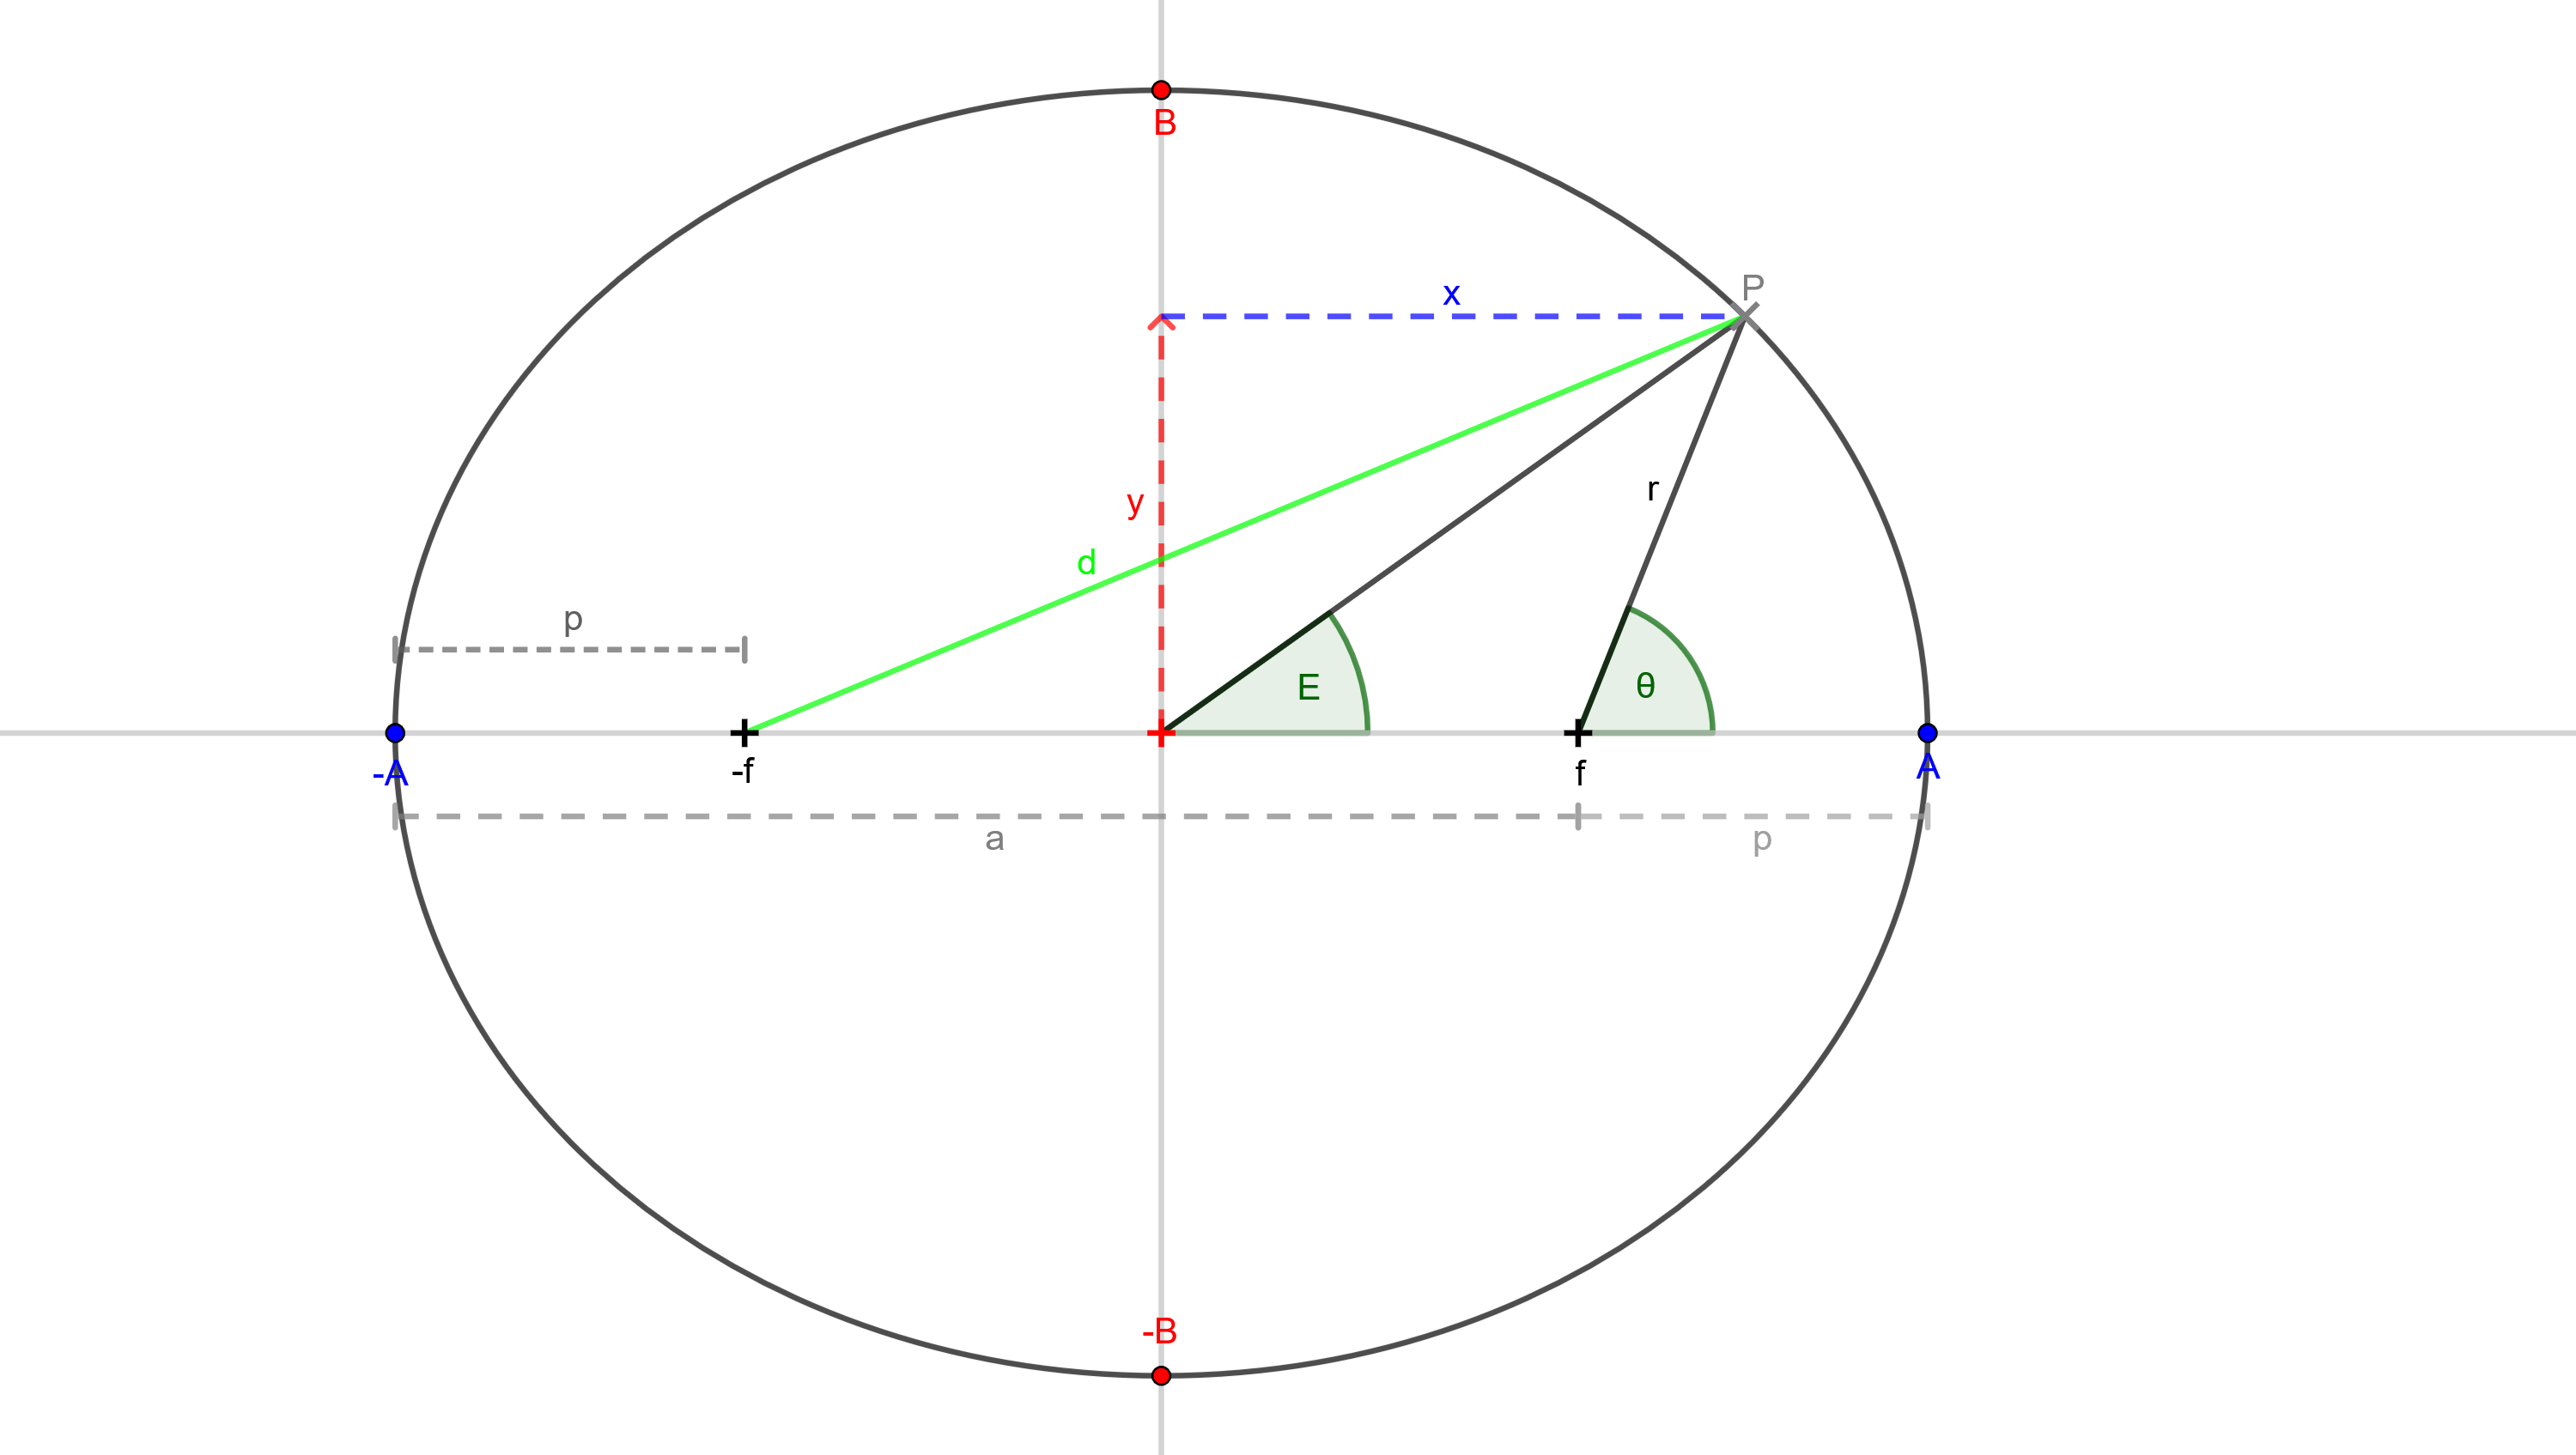
\includegraphics[width=0.8\textwidth]{./img/elipse.png} 
\caption{An Elipse with important values shown} \label{fig:GeometryElipse}
\end{figure}

In figure \ref{fig:GeometryElipse} a point $P$ on the ellipse forms an angle $E$ with the origin and the $x$ axis, this angle is called the \emph{Eccentric Anomaly}.

Also the angle $\theta$ is formed at the ellipse's focus between the point on the ellipse and the axis.

We also define the distances $a$ and $p$ as the apoapsis and periapsis distances respectively.

The semi major axis has been labeled as $A$, so that the total width of the ellipse is $2A$. Also shown on the diagram is the semi minor axis $B$, so the total height of the ellipse is $2B$.

For this text we will take the elliptical eccentricity to be defined as the ratio of the focus and the semi major axis.
\begin{equation}
e = \frac{f}{A} \label{eq:ecentricity}
\end{equation}
\subsection{The Apses}
Before we get any further, we will look at the apses. From figure \ref{fig:GeometryElipse} we can see that

\begin{equation}
p = A - f = A - eA = A(1-e)
\end{equation}

and that
\begin{equation}
a  = A + f = A + eA = A(1+e)
\end{equation}

also

\begin{align}
a+p &= A -f + A +f = 2A \\
a-p &= A + f - A + f = 2f
\end{align}

which can give us the eccentricity as defined by the apses
\begin{equation}
e=\frac{f}{A}=\frac{2f}{2A}=\frac{a-p}{a+p}
\end{equation}

\subsection{Sum of distances from foci and $P$}

One property of an ellipse is that the sum of the distances from any point on the ellipse and the foci is a constant. This fact allows you to draw an ellipse using two pins and a piece of string. We will use this fact and look at two special cases, before looking at the general case and deriving the equation for an ellipse. Before we do we will define what the sum is here.

\begin{equation}
S=d+r \label{eq:elipseConstraint}
\end{equation}

\paragraph{Special Case 1: Point on the $x$ axis}

When the point is at $(A,0)$. The distance $d$ is $f+A$ and the distance $r$ is $A-f$ from the diagram above. So our sum becomes

\begin{equation}
S = d + r = f+A + A-f = 2A \label{eq:ElipseSum}
\end{equation}

\paragraph{Special Case 2: Point on the $y$ axis}

When the point is on the $y$ axis, it is at the point $(0,B)$. The distance $d$ is $\sqrt{f^2+B^2}$ and the distance $r$ is also $\sqrt{f^2+B^2}$ from the diagram above. So our sum is

\begin{equation}
S = 2 \sqrt{f^2+B^2}
\end{equation}

and if the sum is a constant then this will be equal to the value obtained before\footnote{equation \ref{eq:ElipseSum}}.

\begin{equation}
S = 2 \sqrt{f^2+B^2} = 2 A
\end{equation}

and so we now have the relationship between the semi major and minor axes and the focus

\begin{equation}
 A^2=f^2+B^2
\end{equation}

This can also be used to get $B$ in terms of $A$ using the connection to the eccentricity\footnote{equation \ref{eq:ecentricity}}

\begin{align}
B^2&=A^2-f^2\nonumber \\
&=A^2-(eA)^2\nonumber \\
&=A^2(1-e^2)\nonumber \\
\Rightarrow  & B = A\sqrt{1-e^2}
\end{align}

\paragraph{General case}

In general for a point at $(x,y)$ we get the following
\begin{align}
r^2&=(x-f)^2+y^2\\
d^2&=(x+f)^2+y^2
\end{align}

by looking at the triangles formed in figure \ref{fig:GeometryElipse} with hypotenuse being $r$ and $d$ respectively. The sum\footnote{equation \ref{eq:elipseConstraint}} then becomes 

\begin{align}
S=2A&=\sqrt{(x-f)^2+y^2}+\sqrt{(x+f)^2+y^2}\nonumber \\
2A-\sqrt{(x-f)^2+y^2} &= \sqrt{(x+f)^2+y^2}
\end{align}

squaring both sides gives
\begin{align}
\left( 2A-\sqrt{(x-f)^2+y^2} \right)^2 &= (x+f)^2+y^2\nonumber \\
4A^2-4A\sqrt{(x-f)^2+y^2}+(x-f)^2+y^2  &= (x+f)^2+y^2\nonumber \\
4A^2-4A\sqrt{(x-f)^2+y^2}+x^2-2xf+f^2  &= x^2+2xf+f^2\nonumber \\
4A^2-4A\sqrt{(x-f)^2+y^2} &= 4xf\nonumber \\
4A^2-4xf &= 4A\sqrt{(x-f)^2+y^2}\nonumber \\
\frac{4A^2-4xf}{4A} &= \sqrt{(x-f)^2+y^2}\nonumber \\
\sqrt{(x-f)^2+y^2} &=A-\frac{xf}{A}
\end{align}

Squaring both sides gives again gives
\begin{align}
(x-f)^2+y^2 &=\left(A-\frac{xf}{A}\right)^2\nonumber \\
x^2-2xf+f^2+y^2 &=A^2-2\frac{xfA}{A}+\frac{x^2f^2}{A^2}\nonumber \\
x^2-2xf+f^2+y^2 &=A^2-2xf+e^2x^2\nonumber \\
(1-e^2)x^2+y^2 &=A^2-f^2\nonumber \\
(1-e^2)x^2+y^2 &=A^2(1-e^2)\nonumber \\
\frac{(1-e^2)x^2}{A^2(1-e^2)}+\frac{y^2}{A^2(1-e^2)}&=1\nonumber \\
\frac{x^2}{A^2}+\frac{y^2}{B^2}&=1 \label{eq:ElipseCartesian}
\end{align}

Which is the cartesian form of an elipse, there by showing that the elipse does indeed obey the contstraint that the sum of the distances from the foci is a constant.

\paragraph{Polar Form}

Once again returning to figure \ref{fig:GeometryElipse} we can see that 

\begin{align}
x &= f+r\cos \theta \\
y &= r \sin \theta
\end{align}

The sum\footnote{equation \ref{eq:elipseConstraint}} then becomes

\begin{align}
S = 2A &= r + d\nonumber \\
2A -r &= d
\end{align}

We can square both sides to get

\begin{align}
\left(2A -r\right)^2 &= d^2\nonumber \\
4A^2 -4Ar +r^2 &= (x+f)^2+y^2\nonumber \\
&= x^2+2fx+f^2+y^2\nonumber \\
&= \left(f+r \cos \theta\right)^2+2fx+f^2+r^2\sin^2\theta \nonumber \\
&= f^2+2fr \cos \theta + r^2 \cos^2\theta+2f\left(f+r \cos \theta\right)+f^2 \nonumber \\
&+r^2\sin^2\theta \nonumber \\
 &= f^2+2fr \cos \theta +2f^2+2fr \cos\theta+f^2\nonumber \\
&+r^2(\sin^2\theta+\cos^2\theta)\nonumber \\
 &= 4f^2+4fr \cos \theta+r^2\nonumber \\
A^2 -Ar &= f^2+fr \cos \theta\nonumber \\
A^2 -f^2 &= \left( A+f \cos \theta\right) r\nonumber \\
A^2 -e^2A^2 &= \left( A+eA \cos \theta\right) r\nonumber \\
A^2\left(1-e^2\right)&= A\left( 1+e \cos \theta\right) r\nonumber \\
A\left(1-e^2\right)&= \left( 1+e \cos \theta\right) r
\end{align}

Which with some rearranging results in the polar form for the equation of an elipse
\begin{equation}
r = \frac{A\left(1-e^2\right)}{ 1+e \cos \theta}
\end{equation}

\subsection{Relationship between $\theta$ and $E$}

Looking at figure \ref{fig:GeometryElipse} again we can see that $x$ and $y$ can also be given by

\begin{align}
x &= A \cos E \\
y &= B \sin E = A \sqrt{1-e^2} \sin E
\end{align}

We can also see that $r$ can be given by

\begin{align}
r^2 &= (x-f)^2 + y^2\nonumber \\
&= x^2-2xf+f^2 + y^2\nonumber  \\
&= A^2 \cos^2 E-2eA^2\cos E+e^2A^2 + A^2(1-e^2)\sin^2 E\nonumber  \\
\left(\frac{r}{A}\right)^2 &=  \cos^2 E-2e\cos E+e^2 + (1-e^2)\sin^2 E\nonumber  \\
\left(\frac{r}{A}\right)^2 &=  \cos^2 E-2e\cos E+e^2 + \sin^2 E-e^2\sin^2 E\nonumber  \\
\left(\frac{r}{A}\right)^2 &=  \left(\sin^2 E+\cos^2 E\right)-2e\cos E+e^2(1-\sin^2 E)\nonumber  \\
\left(\frac{r}{A}\right)^2 &=  1-2e\cos E+e^2\cos^2 E\nonumber  \\
\left(\frac{r}{A}\right)^2 &=  (1)^2-2(1)(e\cos E)+(e\cos E)^2\nonumber  \\
\left(\frac{r}{A}\right)^2 &=  \left( 1-e\cos E\right)^2
\end{align}

leading to
\begin{equation}
r = A\left( 1-e\cos E\right) \label{eq:radiusVsEccentric Anomaly}
\end{equation}